%This TEX file is for the tables and Figures in paper "Patent Value and %Dynamic R&D choice 
\documentclass[english]{article}
\usepackage{graphicx}
\usepackage{caption}
\usepackage{float}
\usepackage{multirow}
%\usepackage{array}
%\usepackage{adjustbox}
\usepackage{booktabs}
\usepackage{amssymb}
\begin{document}

\section*{Tables and Figures}

\begin{center}
\begin{table}[H]
\label{T1}
\caption{Number of patents in the merged database and matching efficiency}

\begin{centering}
\begin{tabular}{clllllll}
\hline\hline
year & 2001 & 2002 & 2003 & 2004 & 2005 & 2006 & 2007\\
\hline\hline
invention & 1982 & 4462 & 5333 & 7993 & 10100 & 17033 & 19750 \\
utility model & 4202 & 5649 & 7496 & 7798 & 10720 & 15324 & 18212\\
\hline
matching  & 57.10\% & 81.26\% & 96.35\% & 87.20\% & 57.58\% & 67.33\% & 55.67\% \\
\hline
\hline
\end{tabular}
\par\end{centering}
{\small{}Note: matching efficiency refers the ratio of number of invention
patents in the merged data set to the published figure in China Statistical
Yearbook on Science and Technology 2001-2007.}{\small \par}
\end{table}
\par\end{center}


\begin{center}
\begin{table}[H]
\caption{Summary statistics for high-tech and non-high-tech industries}
\label{T2}
\begin{centering}
\begin{tabular}{lllll}
\hline\hline
 & \multicolumn{2}{c}{High-tech} & \multicolumn{2}{c}{Non-high-tech} \\
Variable & Mean & Std. Dev. & Mean & Std. Dev.\\
\hline\hline 
R\&D expenditures & 218.095 & 963.152 & 34.886 & 326.677\\
R\&D/employees & 1.794 & 8.327 & 0.282 & 4.686\\
R\&D/sales & 0.007 & 0.024 & 0.001 & 0.008\\
Invention patents & 0.056 & 0.776 & 0.010 & 0.306\\
Utility patents & 0.083 & 1.058 & 0.028 & 0.376\\
\hline\hline
\end{tabular}
\par\end{centering}
{\small{}Note: the unit of R\&D expenditure is 1,000 yuan (around
150 US dollars).}{\small \par}
\end{table}
\par\end{center}




\begin{center}
\begin{figure}[H]
\label{F1}
\caption{Number of Firms by Innovation Activities} 

\begin{centering}
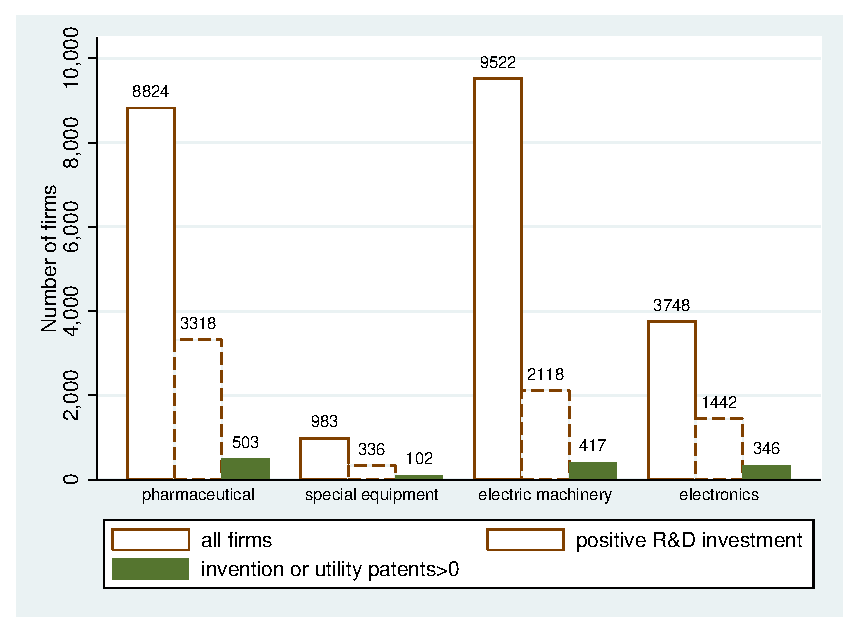
\includegraphics[width=0.8\textwidth]{FirmsCount.eps}
\par\end{centering}
{\small{}Note: numbers are from the final database}{\small \par}
\end{figure}
\par\end{center}

\begin{center}
\begin{figure}[H]
\caption{An Overview of the Theoretical Model}
\label{F2}

\begin{centering}
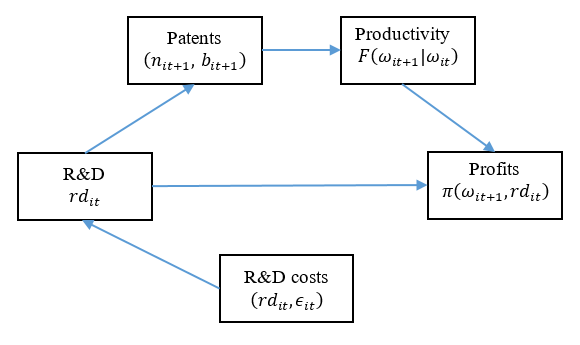
\includegraphics[width=1\textwidth]{Overview.PNG}
\par\end{centering}
\caption*{\small{}Note: $i$ represents firm and $t$ represents year. $rd$ is the R\&D investment, $\epsilon_{it}$ is the firm-year specific cost coefficient, $\omega_{it}$ is the productivity, and $n_{it}$ ($b_{it}$) represents the invention (utility model) patents applications.}{\small \par}
\end{figure}
\par\end{center}




\begin{table}[H]
\centering
\caption{Distribution of patents}
\label{T3}
\begin{tabular}{lccccc}
\hline\hline
Patents counts & 0       & $\geq 1$ & 1      & 2      & $\geq 3$ \\
\hline\hline 
Invention&98.01\% & 1.99\% & 1.22\% & 0.39\% & 0.37\% \\
Utility&95.72\% & 4.28\% & 2.22\% & 0.96\% & 1.10\% \\
Design&97.90\% & 2.10\% & 0.97\% & 0.44\% & 0.69\% \\
\hline\hline
\end{tabular}

{\small{}Note:the percentage represents the share of observations in the specified cohort.}{\small \par}
\end{table}


\begin{table}[H]
\centering
\caption{R\&D and the distribution of patent applications}
\label{T4}
\begin{tabular}{lllll}
\hline\hline 
Previous R\&D & Stats  & invention  & utility  & design \\
\hline\hline 
 0    &mean     & 0.026  & 0.074   & 0.047  \\
      &variance & 0.248  & 0.562   & 0.382  \\
      &max      & 77     & 90      & 40     \\
      &  $P(pat>0)$    & 1.35\% & 3.33\%  & 1.60\% \\
      &N        &   & 34732   &   \\
      \hline
(0, p25]     & mean     & 0.040  & 0.096   & 0.088  \\
        & variance & 0.109  & 0.297   & 1.646  \\
      & max      & 9      & 10      & 48     \\
      &  $P(pat>0)$   & 2.25\% & 4.99\%  & 2.28\% \\
      & N        &    & 3025   &   \\
      \hline 
(p25, p75]   & mean     & 0.084  & 0.178   & 0.121  \\
      & variance & 0.301  & 0.796   & 1.336  \\
      & max      & 17     & 22      & 68     \\
      &  $P(pat>0)$   & 4.46\% & 7.82\%  & 3.92\% \\
      & N        &    & 6051    &   \\
      \hline
(p75,p100]    &mean & 0.187  & 0.413   & 0.177  \\
      & variance & 0.702  & 8.830   & 1.370  \\
      & max      & 20    & 144     & 26     \\
      &  $P(pat>0)$   & 9.23\% & 14.33\% & 5.92\% \\
      & N        &    & 3022    &  \\
\hline\hline
\end{tabular}
\caption*{\small{}Note: p"x" is the x percentile in the distribution of R\&D investment for R\&D$>$0. $P(pat>0)$ is the share of observations with positive patent applications. N is the number of observations.}{\small \par}
\end{table}



\begin{table}[H]
\centering
\caption{Simple correlation between R\&D and Patents}
\label{T5A}
{
\def\sym#1{\ifmmode^{#1}\else\(^{#1}\)\fi}
\begin{tabular}{l*{4}{c}}
\hline\hline
            &\multicolumn{2}{c}{inpat}&\multicolumn{2}{c}{utpat}\\\cmidrule{2-5}
            &\multicolumn{1}{c}{(1)}&\multicolumn{1}{c}{(2)}&\multicolumn{1}{c}{(3)}&\multicolumn{1}{c}{(4)}\\
            &\multicolumn{1}{c}{all}&\multicolumn{1}{c}{invpat$\geq 1$}&\multicolumn{1}{c}{all}&\multicolumn{1}{c}{utipat$\geq 1$}\\
           
\hline
$RD_{t-1}$       &      0.0171\sym{***}&     -0.0117         &      0.0283\sym{***}&      0.0713         \\
            &   (0.00201)         &    (0.0410)         &   (0.00626)         &    (0.0752)         \\
\hline
\(N\)       &       23077         &         738         &       23077         &         843         \\
\(R^{2}\)   &       0.008         &       0.019         &       0.007         &       0.013         \\
\hline\hline
\end{tabular}
}

\caption*{\small{}Note: all regression contain industry, year, and industry-year fixed effects. Results in columns (1) and (3) are obtained using all the sample; columns (2) and (4) display the results using observations with positive patent applications. Standard errors in parentheses.{*} \(p<0.05\), {**} \(p<0.01\), {***} \(p<0.001\)} {\small \par}
\end{table}

\begin{table}[H]
\centering
\caption{Simple correlation between R\&D and log of Patents}
\label{T5B}
{
\def\sym#1{\ifmmode^{#1}\else\(^{#1}\)\fi}
\begin{tabular}{l*{4}{c}}
\hline\hline
  &\multicolumn{2}{c}{$log$(inpat+1)}&\multicolumn{2}{c}{$log$(utpat+1)}\\\cmidrule{2-5}
            &\multicolumn{1}{c}{(1)}&\multicolumn{1}{c}{(2)}&\multicolumn{1}{c}{(3)}&\multicolumn{1}{c}{(4)}\\
            &\multicolumn{1}{c}{all}&\multicolumn{1}{c}{invpat$\geq 1$}&\multicolumn{1}{c}{all}&\multicolumn{1}{c}{utipat$\geq 1$}\\
\hline
$RD_{t-1}$        &     0.00869\sym{***}&     0.00376         &      0.0103\sym{***}&     0.00842         \\
            &  (0.000682)         &   (0.00520)         &  (0.000817)         &   (0.00579)         \\
\hline
\(N\)       &       23077         &         738         &       23077         &         843         \\
\(R^{2}\)   &       0.025         &       0.034         &       0.037         &       0.025         \\
\hline\hline
\end{tabular}
}

\caption*{\small{}Note: all regression contain industry, year, and industry-year fixed effects. Results in columns (1) and (3) are obtained using all the sample; columns (2) and (4) display the results using observations with positive patent applications. Standard errors in parentheses.{*} \(p<0.05\), {**} \(p<0.01\), {***} \(p<0.001\)} {\small \par}
\end{table}

\begin{table}[H]
\centering
\caption{Distribution of R\&D conditional on patents outcome}
\label{T6}
\begin{tabular}{lclll}
\hline\hline
                                & \multicolumn{2}{c}{Invention} & \multicolumn{2}{c}{Utility}   \\\cmidrule{2-5}
Stats                           & 0      & inpat\textgreater0 & 0      & utpat\textgreater0 \\
\hline\hline
mean                            & 1.53    & 3.36                & 1.53   & 3.33                \\
variance                  & 6.45    & 10.16               & 6.44   & 10.41               \\
mean(R\&D$>0$)           & 5.17    & 5.94                & 5.16   & 5.98                \\
variance(R\&D$>0$) & 2.97    & 2.81                & 2.96   & 2.84                \\
prob(R\&D$>0$)                            & 29.7\%  & 60.2\%              & 29.7\% & 55.6\%  \\
\hline\hline                 
\end{tabular}
\end{table}

\begin{table}[H]
\centering
\caption{Impact of R\&D and patents on productivity: extensive margin}
\label{T8}
{
\def\sym#1{\ifmmode^{#1}\else\(^{#1}\)\fi}
\begin{tabular}{l*{5}{c}}
\hline\hline
           &\multicolumn{5}{c}{Dependent variable: $lp_{t+1}$} \\\cmidrule{2-6}
            &\multicolumn{1}{c}{(1)}&\multicolumn{1}{c}{(2)}&\multicolumn{1}{c}{(3)}&\multicolumn{1}{c}{(4)}&\multicolumn{1}{c}{(5)}\\

\hline
$lp_{t}$        &       0.598\sym{***}&       0.597\sym{***}&       0.597\sym{***}&       0.597\sym{***}&       0.597\sym{***}\\
            &   (0.00806)         &   (0.00806)         &   (0.00807)         &   (0.00806)         &   (0.00807)         \\
$rd_{t}$      &      0.0877\sym{***}&      0.0787\sym{***}&      0.0771\sym{***}&      0.0851\sym{***}&      0.0766\sym{***}\\
            &    (0.0124)         &    (0.0127)         &    (0.0129)         &    (0.0126)         &    (0.0129)         \\
$rd_{t}\times inpat_{t+1}$        &                     &       0.131\sym{***}&       0.123\sym{***}&                     &       0.133\sym{**} \\
            &                     &    (0.0346)         &    (0.0369)         &                     &    (0.0440)         \\
$rd_{t}\times utpat_{t+1}$        &                     &                     &      0.0313         &                     &      0.0424         \\
            &                     &                     &    (0.0365)         &                     &    (0.0435)         \\
$rd_{t}\times inpat_{t+1} \times utpat_{t+1} $     &                     &                     &                     &       0.124\sym{*}  &     -0.0430         \\
            &                     &                     &                     &    (0.0491)         &    (0.0774)         \\
\hline
\(N\)       &       11859         &       11859         &       11859         &       11859         &       11859         \\
\(R^{2}\)   &       0.531         &       0.532         &       0.532         &       0.531         &       0.532         \\
\hline\hline
\end{tabular}
}

\caption*{\small{}all regression contain industry, year, and industry-year fixed effects. Standard errors in parentheses.{*} \(p<0.05\), {**} \(p<0.01\), {***} \(p<0.001\)} {\small \par}
\end{table}

\begin{table}[H]
\centering
\caption{Impact of R\&D and patents on productivity: intensive margin}
\label{T9}
{
\def\sym#1{\ifmmode^{#1}\else\(^{#1}\)\fi}
\begin{tabular}{l*{5}{c}}
\hline\hline
            &\multicolumn{5}{c}{Dependent variable: $lp_{t+1}$}\\\cmidrule{2-6}
            &\multicolumn{1}{c}{(1)}&\multicolumn{1}{c}{(2)}&\multicolumn{1}{c}{(3)}&\multicolumn{1}{c}{(4)}&\multicolumn{1}{c}{(5)}\\
\hline
 $lp_{t}$        &       .598\sym{***}&       .547\sym{***}&       .616\sym{***}&       .623\sym{***}&       .614\sym{***}\\
            &   (.00806)         &    (.0405)         &    (.0554)         &    (.0561)         &    (.0554)         \\
$rd_{t}$      &      .0877\sym{***}&       .188\sym{*}  &      0.0604         &       0.142         &      0.0147         \\
            &    (0.0124)         &    (0.0794)         &     (0.111)         &    (0.0969)         &     (0.135)         \\
$rd_{t}\times inpat_{t+1}$    &                     &     -0.0116         &      0.0589         &                     &      0.0613         \\
            &                     &    (0.0329)         &    (0.0417)         &                     &    (0.0432)         \\
$rd_{t}\times utpat_{t+1}$    &                     &                     &    -0.00437         &                     &      0.0119         \\
            &                     &                     &   (0.00375)         &                     &    (0.0183)         \\
$rd_{t}\times inpat_{t+1} \times utpat_{t+1} $  &                     &                     &                     &   .000016        &    -0.00128         \\
            &                     &                     &                     &  (.000126)         &   (.00147)         \\
\hline
\(N\)       &       11859         &         474         &         138         &         138         &         138         \\
\(R^{2}\)   &       0.531         &       0.540         &       0.686         &       0.680         &       0.687         \\
\hline\hline
\end{tabular}
}

\caption*{\small{}all regression contain industry, year, and industry-year fixed effects. } {\small \par}
\end{table}

\begin{table}[H]
\centering
\caption{Distribution of patent applications conditional on R\&D decision}
\label{T10}
\begin{tabular}{lllll}
\hline\hline
Industries     & $p(0,0)$& $p(1,0)$& $p(0,1)$ & $p(1,1)$ \\
\hline\hline
pharmaceutical & 0.903 & 0.085 & 0.007 & 0.005  \\
equipment      & 0.826 & 0.012 & 0.115 & 0.047 \\
electronics    & 0.899 & 0.009 & 0.069 & 0.023 \\
machinery      & 0.857 & 0.015 & 0.094 & 0.035 \\
\hline\hline 
\multicolumn{5}{l}{\footnotesize Note: $p(x,y)=Prob(n_{t+1}=x, b_{t+1}=y|d_{t}=1)$.}
\end{tabular}
\end{table}

\begin{table}[H]
\centering
\caption{Estimates of demand elasticities}
\label{T11}
\begin{tabular}{lllll}
\toprule 
industry & pharmaceutical & equipment & electronics & machinery \\
\midrule 
$\hat{\sigma}$ &  5.926 & 5.043 & 6.341 & 5.415 \\

$\frac{\hat{\sigma}}{\hat{\sigma}-1}$ & 1.203  & 1.247  & 1.187  & 1.227 \\

\bottomrule 
\end{tabular}
\end{table}

\begin{table}[H]
\centering
\caption{Estimates of productivity evolution equation and cost function}
\label{T12}
\def\sym#1{\ifmmode^{#1}\else\(^{#1}\)\fi}
\begin{tabular}{lllll}
\toprule 
 & \multicolumn{2}{c}{cubic parameterization}\\
\midrule
\multicolumn{5}{l}{\textit{Productivity evolution:}}\\
$rd_t$                    & .00435\sym{**}  & (2.90) \\
$n_{t+1} \times rd_t$     &  .0145\sym{**} & (2.90) \\
$b_{t+1} \times rd_t $     & .0137\sym{*} & (2.76) \\
$\phi_{t}$             & .824\sym{**}  & (14.96)  \\
$\phi_{t}^{2}$         & .503\sym{**} & (2.69)  \\
$\phi_{t}^{3}$         & -1.135\sym{**}& (-14.26)\\
\midrule 
$\rho_{0}$:               &  &  &  & \\
common part               &.0295\sym{**} & (8.34) \\
Pharmaceutical            & -.0144\sym{*}&(-3.90) \\
Electronics               & -.0132\sym{**} &(-3.61)\\
Electric Machinery       & -.0116\sym{**} &(-2.92) \\ 
$\sigma_{\varepsilon}$ & \multicolumn{2}{c}{.10} \\
\midrule 
\multicolumn{5}{l}{\textit{Cost function:}} \\
$k$                      & -.0299\sym{**}& (-25.82)   \\       
$a\in\left(10,\,19\right)$  & .0740\sym{**} &(12.62)\\
$a\in\left(20,\,49\right)$  & 0.111\sym{**}&(12.88)   \\
$a\geq50$                &.149\sym{**}  & (7.84) \\
\midrule              
sample size & \multicolumn{4}{c}{22492}\tabularnewline
\bottomrule
\end{tabular}


\caption*{\small{}Note:$\left(\partial\omega_{t+1}/\partial\omega_{t}\right)_{max}$
is the maximum partial derivative of $\omega_{t+1}$ with respect
to $\omega_{t}$. T statistics are in parentheses; {*} p$<$0.05, {*}{*}
p$<$0.01. }{\small \par}
\end{table}


\Section*{Appendix}
\setcounter{table}{0} %reset the table counter
\renewcommand{\tablename}{Table} % Set the tablename to Panel, instead of Table
\renewcommand{\thetable}{\Alph{table}} \ % Setting the table number output to letters
\begin{table}[H]
\centering
\caption{Estimates of productivity evolution equation: supplementary results}
\label{TA1}
{
\def\sym#1{\ifmmode^{#1}\else\(^{#1}\)\fi}
\begin{tabular}{l*{1}{cc}}
\hline\hline
\multicolumn{3}{c}{productivity evolution equation  }\\
\hline 
$\omega_t$       &       0.826\sym{**}&     (17.13)\\
$\omega_t^2$     &        0.300\sym{**}&     (15.87)\\

$rd_t$    &     0.00505\sym{**}&      (3.35)\\

$rd_t\times n_{t+1}$      &      0.0153\sym{**}&      (3.04)\\
$rd_t \times b_{t+1}$      &     0.0142\sym{*} &      (2.85)\\
$\beta_k$                  & -0.308\sym{**}    &     (-25.71)\\
\hline
\(N\)       &       22492        &            \\
\hline\hline
\end{tabular}
}

\caption*{\small{}Note:$\left(\partial\omega_{t+1}/\partial\omega_{t}\right)_{max}$
is the maximum partial derivative of $\omega_{t+1}$ with respect
to $\omega_{t}$. T statistics are in parentheses; {*} p$<$0.05, {*}{*}
p$<$0.01. }{\small \par}
\end{table}

\end{document}